% !TeX program = xelatex
% RADiCAL Poster - Coe College themed (Gemini beamerposter theme)
% Base theme: https://github.com/anishathalye/gemini
% Requires: beamerthemegemini.sty + beamercolorthemegemini.sty (Coe colors) in the same directory.
% Compile with xelatex or lualatex.

\documentclass[final]{beamer}

\usepackage[T1]{fontenc}
\usepackage[size=custom,width=121.92,height=91.44,scale=1.0]{beamerposter}
\usetheme{gemini}
\setbeamerfont{title}{family=\sffamily, series=\bfseries, size=\fontsize{60}{72}}
\usecolortheme{gemini}
\usepackage{graphicx}
\usepackage{booktabs}
\usepackage{tikz}
\usepackage{subcaption}
\usepackage[style=numeric, backend=biber, sorting=none, maxbibnames=3]{biblatex}
\addbibresource{poster.bib}

% Scalable OpenType math font so big symbols (sqrt, X_0, superscripts) render
% at any poster size without the "OMX/cmex size not available" substitution warning.
\usepackage{unicode-math}
\setmathfont{latinmodern-math.otf}

% ====================
% Lengths
% ====================

\newlength{\sepwidth}
\newlength{\colwidth}
\setlength{\sepwidth}{0.025\paperwidth}
\setlength{\colwidth}{0.3\paperwidth}

\newcommand{\separatorcolumn}{\begin{column}{\sepwidth}\end{column}}

% ====================
% Title
% ====================

\title{The RADiCAL Module: An Ultracompact, Radiation-Hard Calorimeter for Future Colliders}

\author{Walker Law$^{\text{1}}$, Cris Cano$^{\text{1}}$, Ruben Perez$^{\text{2}}$, James Wetzel$^{\text{1,3}}$}

\institute[shortinst]{$^{\text{1}}$Coe College, Cedar Rapids, IA 52402\; $^{\text{2}}$Georgetown University, Washington, D.C. 20007\; $^{\text{3}}$University of Iowa, Iowa City, IA 52242}

% ====================
% Footer (optional)
% ====================

\footercontent{
  \raisebox{.8ex}{\href{mailto:}{wllaw23@coe.edu}}
  \hfill
  \raisebox{.8ex}{\href{https://github.com/walker-law/RADiCAL2026}{github.com/walker-law/RADiCAL2026}}
  \hfill
  \raisebox{0.8ex}{\href{https://linkedin.com/in/walker-law}{linkedin.com/in/walker-law}}
}

% ====================
% Logo (optional)
% ====================

\logoleft{%
  \raisebox{-0.5\height}{
\includegraphics[height=8cm]{logos/CoeLogo.png}}%
  \hspace{2.5cm}%
  \raisebox{-0.5\height}{
\includegraphics[height=8cm]{logos/University-of-Iowa-Logo.png}}%
}
\logoright{%
  \raisebox{-0.5\height}{
\includegraphics[height=8cm]{logos/CERN_logo_outline.jpg}}%
  \hspace{7.5cm}%
  \raisebox{-0.5\height}{
\includegraphics[height=8cm]{logos/Seal_of_the_Department_of_Energy.jpg}}%
}

% ====================
% Body
% ====================
\begin{document}
\large

\addtobeamertemplate{headline}{}
{
% \begin{tikzpicture}[remember picture,overlay]
%   \node [anchor=north west, inner sep=3cm] at ([xshift=-2.25cm,yshift=.25cm]current page.north west)
%     {
\includegraphics[height=6cm]{logos/CoeLogo.png}};
%   \node [anchor=north east, inner sep=3cm] at ([xshift=3cm,yshift=0cm]current page.north east)
%     {\includegraphics[height=5cm]{logos/CollaborationLogo.png}};
% \end{tikzpicture}
}

\begin{frame}[t]
\begin{columns}[t]
\separatorcolumn








% ===================== COLUMN 1 =====================
\begin{column}{\colwidth}

\begin{exampleblock}{\Large Abstract}
  \normalsize
  Future particle colliders, such as the FCC-hh, pose significant challenges for detectors as increased luminosity will lead to more particle pile-up. To create suitable particle detectors for these conditions, the RADiCAL project aims to reach $\sigma_t \leq 10$ ps timing resolution, $\sigma_E/E\leq 10\%$ energy resolution, and $1$ mm position resolution in a finger-sized calorimeter. RADiCAL achieves this as a sampling ``shashlik''-type calorimeter, which alternates between LYSO scintillating crystal and tungsten. However, the RADiCAL module allows for the swapping of scintillating materials, wavelength shifting (WLS) materials, dense absorbing materials, and electronics. This allows for the direct comparison between high-energy physics equipment. We present results from a May 2023 CERN beam test with 5--120 GeV electrons, achieving $\sigma_t \approx 37$ ps at 150 GeV; consistent with previously published RADiCAL benchmarks and validated by Geant4 simulation.
\end{exampleblock}

\begin{block}{\Large Project Goals}
  \normalsize
  \begin{itemize}
    \item 10 ps EM-shower timing resolution, 1 mm position resolution, and 10\%/$\sqrt{\text{GeV}}$ stochastic energy term
    \item Enable 4D/5D calorimetry in a compact, finger-sized package
    \item RADiCAL to become a ``standard candle" to directly compare high-energy physics materials and electronics to one another
    \item Array of RADiCAL modules as a primary detector for $\eta \geq 1.5$ pseudorapidity regions where radiation-hardness and accurate calorimetry are required
  \end{itemize}
  \begin{figure}
    \centering
    \vspace{-1.25cm}
    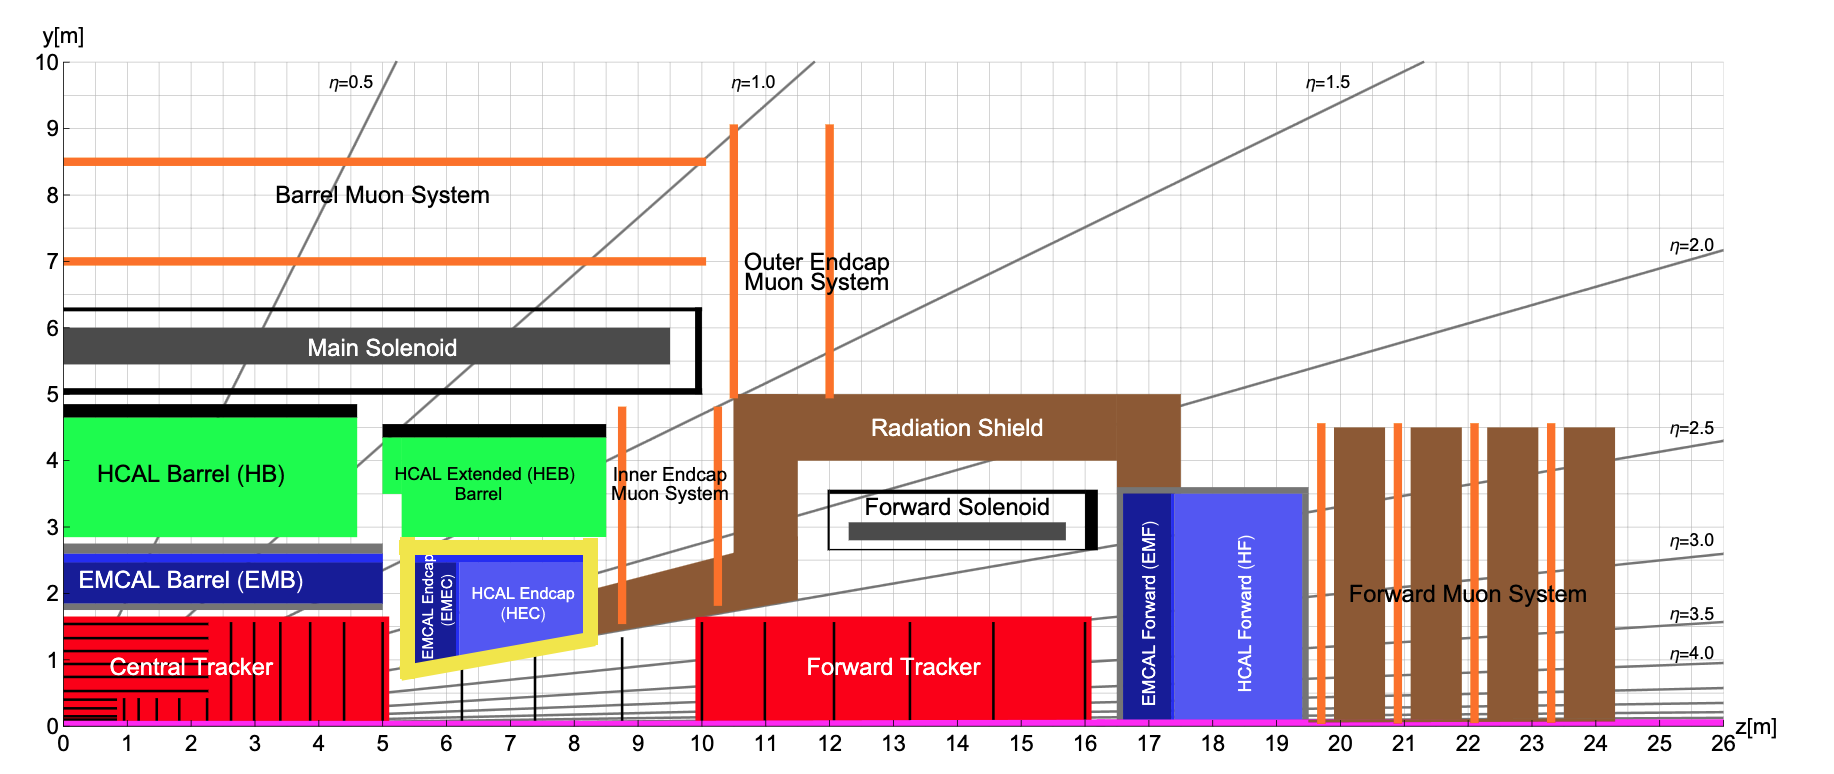
\includegraphics[width=.95\linewidth]{FCCcrosssection.png}
    \vspace{-.5cm}
    \caption{Example FCC-hh detector layout. The EMEC endcap region ($1.48<|\eta|<2.50$) outlined in yellow motivates RADiCAL's target pseudorapidity range. Sourced from \cite{aleksa2019calorimeters}.}
  \end{figure}
\end{block}

\begin{block}{\Large RADiCAL Module}
  \normalsize
  \begin{itemize}
    \item Shashlik-style sampling calorimeter alternating between LYSO scintillating crystal and tungsten
    \item 5 quartz capillaries --- one in the center doped with WLS through entire length, four in each corner doped with WLS only at shower maximum
    \item Quartz capillaries permeate through entire length of calorimeter, guiding WLS photons via TIR to SiPMs on upstream and downstream ends of each capillary
    \item High gain (HG) and low gain (LG) SiPMs on upstream and downstream ends. High gain reduces time-walk for sharp timing measurements, whereas low gain enables signal integration for energy measurements
    \item Assembled to 25 $X_0$ long and contains most of the Molière radius ($R_M\approx13$ mm)
  \end{itemize}
  \begin{figure}
    \vspace{-1cm}
    \centering
    \begin{minipage}[b]{.52\linewidth}
      \centering
      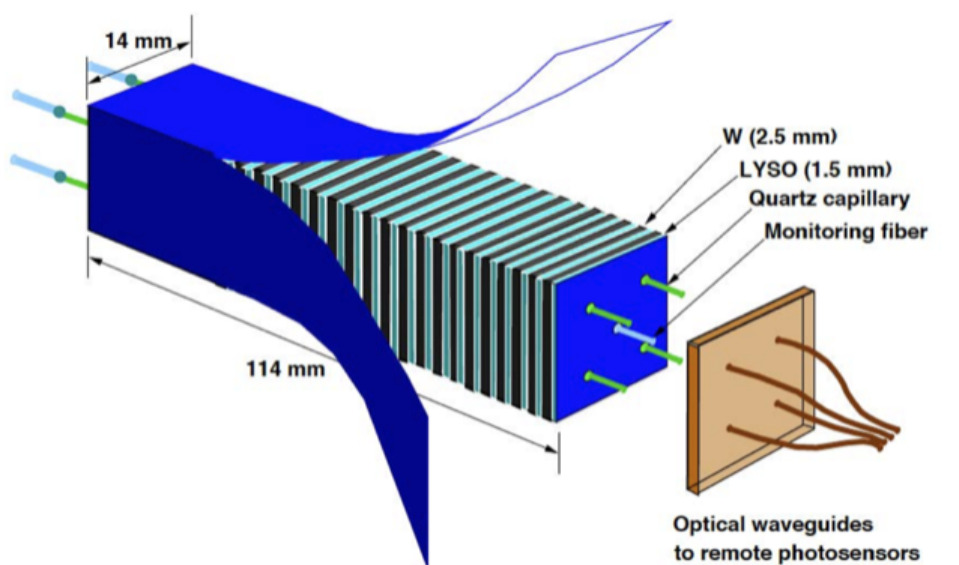
\includegraphics[width=\linewidth]{RADiCALdiagram.jpg}
      \vspace{.25cm}
      \captionof{figure}{Diagram of the RADiCAL module. Sourced from~\cite{wetzel2023beamtest}.}
    \end{minipage}
    \hfill
    \begin{minipage}[b]{.47\linewidth}
      \centering
      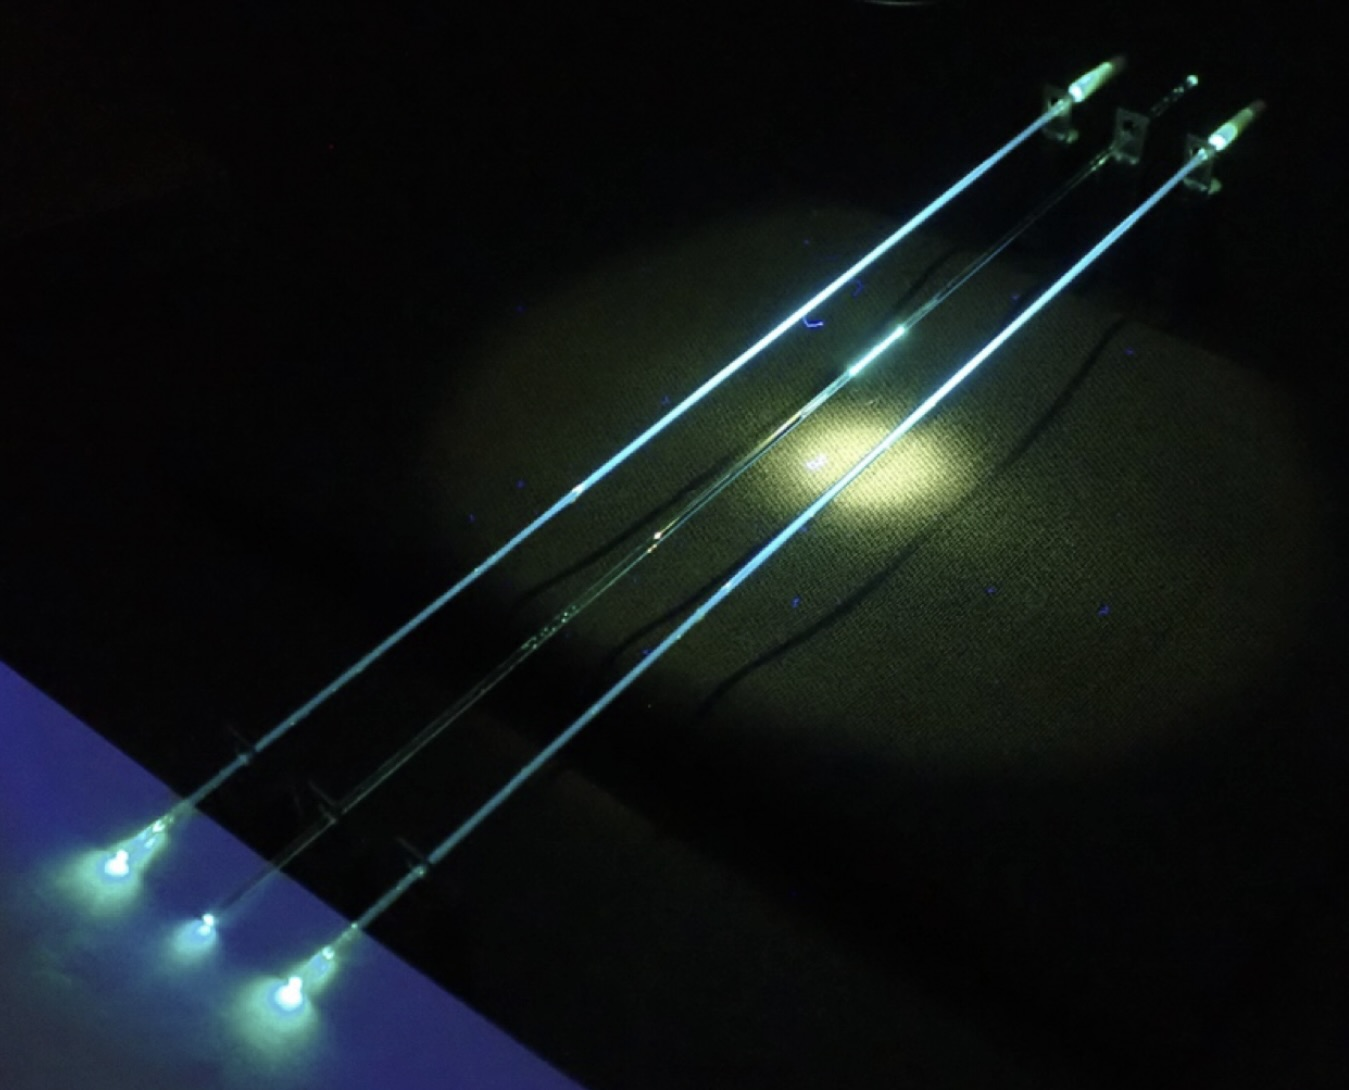
\includegraphics[width=\linewidth]{capillaries.jpeg}
      \captionof{figure}{WLS-doped quartz capillaries lit up. Sourced from \cite{wetzel2023beamtest}.}
    \end{minipage}
    \vspace{-1cm}
  \end{figure}
\end{block}

\end{column}

\separatorcolumn









% ===================== COLUMN 2 =====================
\begin{column}{\colwidth}

\begin{alertblock}{\Large Experiment}
  \normalsize
  \begin{itemize}
    \item Used H2 beamline in CERN's North Area for high-energy electron source
    \item Acquired data with 5, 10, 20, 50, 100, and 120 GeV electrons, with 1,000,000 events per energy
    \item Waveforms digitized at 5 GS/s using CAEN DT5742 / DRS4
    \item MCP used for fast timing resolution reference ($\sigma_t \approx 10$ ps) \cite{wetzel2023beamtest}
  \end{itemize}
  
  \begin{figure}
    \includegraphics[width=.7\linewidth]{experimentalsetup.JPG}
    \vspace{-.5cm}
    \caption{Photograph of the RADiCAL experimental setup. The beam enters from the left (source out of frame) and travels through coincidence scintillators, the multi-channel plate (MCP), the RADiCAL module under a blue light shield, and then the Pb-glass calorimeter.}
  \end{figure} 
\end{alertblock}

\begin{alertblock}{\Large Simulation}
  \normalsize
  \begin{itemize}
  \item Geant4 used to simulate the exact conditions of the real-life experiment
  \item Simulated at 5, 10, 20, 25, 50, and 120 GeV with \textasciitilde100,000 [NOT ACCURATE YET] events per energy 
  \end{itemize}
\end{alertblock}

\begin{block}{\Large Experiment and Simulation Alignment}
  \normalsize
  \begin{itemize}
  \item Experimental 33,200 photons/MeV LYSO photon production is proportionally scaled down to 33.2 photons/MeV in simulation
  \item 
  \end{itemize}
\end{block}
\end{column}

\separatorcolumn









% ===================== COLUMN 3 =====================
\begin{column}{\colwidth}

\begin{block}{\Large Results}
  \normalsize

\end{block}

\begin{exampleblock}{\Large Conclusions}
  \normalsize

\end{exampleblock}

\begin{block}{\Large Future Work}
  \normalsize
  \begin{itemize}
    \item Vary RADiCAL shape and size to optimize timing, energy, and position resolution 
    \item Continue experiments and simulations with various scintillatiing, WLS, and electronic components for direct comparisons
    \item Assemble an array of several RADiCAL modules to study their collective timing and position resolution
  \end{itemize}
\end{block}

\begin{block}{\Large References}
  \small
  \nocite{perezlara2024radical}
  \printbibliography[heading=none]
\end{block}

\begin{block}{\Large Acknowledgments}
  \small
  We would like to thank Coe College, University of Iowa, and CERN for the use of their facilities and computational resources. We also thank the U.S. Department of Energy for the funding of this project under Award Number\\DE-SC0026349.
\end{block}

\end{column}

\separatorcolumn
\end{columns}
\end{frame}

\end{document}